% Options for packages loaded elsewhere
\PassOptionsToPackage{unicode}{hyperref}
\PassOptionsToPackage{hyphens}{url}
%
\documentclass[
]{article}
\usepackage{amsmath,amssymb}
\usepackage{iftex}
\ifPDFTeX
  \usepackage[T1]{fontenc}
  \usepackage[utf8]{inputenc}
  \usepackage{textcomp} % provide euro and other symbols
\else % if luatex or xetex
  \usepackage{unicode-math} % this also loads fontspec
  \defaultfontfeatures{Scale=MatchLowercase}
  \defaultfontfeatures[\rmfamily]{Ligatures=TeX,Scale=1}
\fi
\usepackage{lmodern}
\ifPDFTeX\else
  % xetex/luatex font selection
\fi
% Use upquote if available, for straight quotes in verbatim environments
\IfFileExists{upquote.sty}{\usepackage{upquote}}{}
\IfFileExists{microtype.sty}{% use microtype if available
  \usepackage[]{microtype}
  \UseMicrotypeSet[protrusion]{basicmath} % disable protrusion for tt fonts
}{}
\makeatletter
\@ifundefined{KOMAClassName}{% if non-KOMA class
  \IfFileExists{parskip.sty}{%
    \usepackage{parskip}
  }{% else
    \setlength{\parindent}{0pt}
    \setlength{\parskip}{6pt plus 2pt minus 1pt}}
}{% if KOMA class
  \KOMAoptions{parskip=half}}
\makeatother
\usepackage{xcolor}
\usepackage[margin=1in]{geometry}
\usepackage{color}
\usepackage{fancyvrb}
\newcommand{\VerbBar}{|}
\newcommand{\VERB}{\Verb[commandchars=\\\{\}]}
\DefineVerbatimEnvironment{Highlighting}{Verbatim}{commandchars=\\\{\}}
% Add ',fontsize=\small' for more characters per line
\usepackage{framed}
\definecolor{shadecolor}{RGB}{248,248,248}
\newenvironment{Shaded}{\begin{snugshade}}{\end{snugshade}}
\newcommand{\AlertTok}[1]{\textcolor[rgb]{0.94,0.16,0.16}{#1}}
\newcommand{\AnnotationTok}[1]{\textcolor[rgb]{0.56,0.35,0.01}{\textbf{\textit{#1}}}}
\newcommand{\AttributeTok}[1]{\textcolor[rgb]{0.13,0.29,0.53}{#1}}
\newcommand{\BaseNTok}[1]{\textcolor[rgb]{0.00,0.00,0.81}{#1}}
\newcommand{\BuiltInTok}[1]{#1}
\newcommand{\CharTok}[1]{\textcolor[rgb]{0.31,0.60,0.02}{#1}}
\newcommand{\CommentTok}[1]{\textcolor[rgb]{0.56,0.35,0.01}{\textit{#1}}}
\newcommand{\CommentVarTok}[1]{\textcolor[rgb]{0.56,0.35,0.01}{\textbf{\textit{#1}}}}
\newcommand{\ConstantTok}[1]{\textcolor[rgb]{0.56,0.35,0.01}{#1}}
\newcommand{\ControlFlowTok}[1]{\textcolor[rgb]{0.13,0.29,0.53}{\textbf{#1}}}
\newcommand{\DataTypeTok}[1]{\textcolor[rgb]{0.13,0.29,0.53}{#1}}
\newcommand{\DecValTok}[1]{\textcolor[rgb]{0.00,0.00,0.81}{#1}}
\newcommand{\DocumentationTok}[1]{\textcolor[rgb]{0.56,0.35,0.01}{\textbf{\textit{#1}}}}
\newcommand{\ErrorTok}[1]{\textcolor[rgb]{0.64,0.00,0.00}{\textbf{#1}}}
\newcommand{\ExtensionTok}[1]{#1}
\newcommand{\FloatTok}[1]{\textcolor[rgb]{0.00,0.00,0.81}{#1}}
\newcommand{\FunctionTok}[1]{\textcolor[rgb]{0.13,0.29,0.53}{\textbf{#1}}}
\newcommand{\ImportTok}[1]{#1}
\newcommand{\InformationTok}[1]{\textcolor[rgb]{0.56,0.35,0.01}{\textbf{\textit{#1}}}}
\newcommand{\KeywordTok}[1]{\textcolor[rgb]{0.13,0.29,0.53}{\textbf{#1}}}
\newcommand{\NormalTok}[1]{#1}
\newcommand{\OperatorTok}[1]{\textcolor[rgb]{0.81,0.36,0.00}{\textbf{#1}}}
\newcommand{\OtherTok}[1]{\textcolor[rgb]{0.56,0.35,0.01}{#1}}
\newcommand{\PreprocessorTok}[1]{\textcolor[rgb]{0.56,0.35,0.01}{\textit{#1}}}
\newcommand{\RegionMarkerTok}[1]{#1}
\newcommand{\SpecialCharTok}[1]{\textcolor[rgb]{0.81,0.36,0.00}{\textbf{#1}}}
\newcommand{\SpecialStringTok}[1]{\textcolor[rgb]{0.31,0.60,0.02}{#1}}
\newcommand{\StringTok}[1]{\textcolor[rgb]{0.31,0.60,0.02}{#1}}
\newcommand{\VariableTok}[1]{\textcolor[rgb]{0.00,0.00,0.00}{#1}}
\newcommand{\VerbatimStringTok}[1]{\textcolor[rgb]{0.31,0.60,0.02}{#1}}
\newcommand{\WarningTok}[1]{\textcolor[rgb]{0.56,0.35,0.01}{\textbf{\textit{#1}}}}
\usepackage{graphicx}
\makeatletter
\def\maxwidth{\ifdim\Gin@nat@width>\linewidth\linewidth\else\Gin@nat@width\fi}
\def\maxheight{\ifdim\Gin@nat@height>\textheight\textheight\else\Gin@nat@height\fi}
\makeatother
% Scale images if necessary, so that they will not overflow the page
% margins by default, and it is still possible to overwrite the defaults
% using explicit options in \includegraphics[width, height, ...]{}
\setkeys{Gin}{width=\maxwidth,height=\maxheight,keepaspectratio}
% Set default figure placement to htbp
\makeatletter
\def\fps@figure{htbp}
\makeatother
\setlength{\emergencystretch}{3em} % prevent overfull lines
\providecommand{\tightlist}{%
  \setlength{\itemsep}{0pt}\setlength{\parskip}{0pt}}
\setcounter{secnumdepth}{5}
\ifLuaTeX
  \usepackage{selnolig}  % disable illegal ligatures
\fi
\usepackage{bookmark}
\IfFileExists{xurl.sty}{\usepackage{xurl}}{} % add URL line breaks if available
\urlstyle{same}
\hypersetup{
  pdftitle={R Notebook},
  pdfauthor={Mandip Chaudhary (17)},
  hidelinks,
  pdfcreator={LaTeX via pandoc}}

\title{R Notebook}
\author{Mandip Chaudhary (17)}
\date{}

\begin{document}
\maketitle

{
\setcounter{tocdepth}{3}
\tableofcontents
}
\begin{enumerate}
\def\labelenumi{\arabic{enumi}.}
\setcounter{enumi}{6}
\tightlist
\item
  Do the following in R Studio using ``airquality'' dataset of R with R
  script to knit PDF output.
\end{enumerate}

\begin{enumerate}
\def\labelenumi{\alph{enumi}.}
\tightlist
\item
  Perform test of normality of ``Temp'' variable by each category of
  ``Month'' variable and interpret all the results carefully
\end{enumerate}

\begin{Shaded}
\begin{Highlighting}[]
\CommentTok{\# Load necessary libraries}
\FunctionTok{library}\NormalTok{(car)  }\CommentTok{\# For Levene\textquotesingle{}s test}
\end{Highlighting}
\end{Shaded}

\begin{verbatim}
## Loading required package: carData
\end{verbatim}

\begin{Shaded}
\begin{Highlighting}[]
\FunctionTok{library}\NormalTok{(rstatix)  }\CommentTok{\# For statistical tests}
\end{Highlighting}
\end{Shaded}

\begin{verbatim}
## 
## Attaching package: 'rstatix'
\end{verbatim}

\begin{verbatim}
## The following object is masked from 'package:stats':
## 
##     filter
\end{verbatim}

\begin{Shaded}
\begin{Highlighting}[]
\FunctionTok{library}\NormalTok{(ggplot2)  }\CommentTok{\# For visualization}

\CommentTok{\# Load the dataset}
\FunctionTok{data}\NormalTok{(airquality)}

\CommentTok{\# Convert Month to factor for better analysis}
\NormalTok{airquality}\SpecialCharTok{$}\NormalTok{Month }\OtherTok{\textless{}{-}} \FunctionTok{factor}\NormalTok{(airquality}\SpecialCharTok{$}\NormalTok{Month, }
                          \AttributeTok{levels =} \DecValTok{5}\SpecialCharTok{:}\DecValTok{9}\NormalTok{,}
                          \AttributeTok{labels =} \FunctionTok{c}\NormalTok{(}\StringTok{"May"}\NormalTok{, }\StringTok{"June"}\NormalTok{, }\StringTok{"July"}\NormalTok{, }\StringTok{"August"}\NormalTok{, }\StringTok{"September"}\NormalTok{))}

\CommentTok{\# a. Test of normality for each month}
\CommentTok{\# Shapiro{-}Wilk test for each month}
\NormalTok{normality\_tests }\OtherTok{\textless{}{-}}\NormalTok{ airquality }\SpecialCharTok{\%\textgreater{}\%}
  \FunctionTok{group\_by}\NormalTok{(Month) }\SpecialCharTok{\%\textgreater{}\%}
  \FunctionTok{shapiro\_test}\NormalTok{(Temp)}

\FunctionTok{print}\NormalTok{(normality\_tests)}
\end{Highlighting}
\end{Shaded}

\begin{verbatim}
## # A tibble: 5 x 4
##   Month     variable statistic     p
##   <fct>     <chr>        <dbl> <dbl>
## 1 May       Temp         0.948 0.135
## 2 June      Temp         0.972 0.583
## 3 July      Temp         0.946 0.119
## 4 August    Temp         0.964 0.369
## 5 September Temp         0.951 0.183
\end{verbatim}

\begin{Shaded}
\begin{Highlighting}[]
\CommentTok{\# Visual check of normality using Q{-}Q plots}
\FunctionTok{ggplot}\NormalTok{(airquality, }\FunctionTok{aes}\NormalTok{(}\AttributeTok{sample =}\NormalTok{ Temp)) }\SpecialCharTok{+}
  \FunctionTok{geom\_qq}\NormalTok{() }\SpecialCharTok{+}
  \FunctionTok{geom\_qq\_line}\NormalTok{() }\SpecialCharTok{+}
  \FunctionTok{facet\_wrap}\NormalTok{(}\SpecialCharTok{\textasciitilde{}}\NormalTok{Month) }\SpecialCharTok{+}
  \FunctionTok{labs}\NormalTok{(}\AttributeTok{title =} \StringTok{"Q{-}Q Plots of Temperature by Month"}\NormalTok{)}
\end{Highlighting}
\end{Shaded}

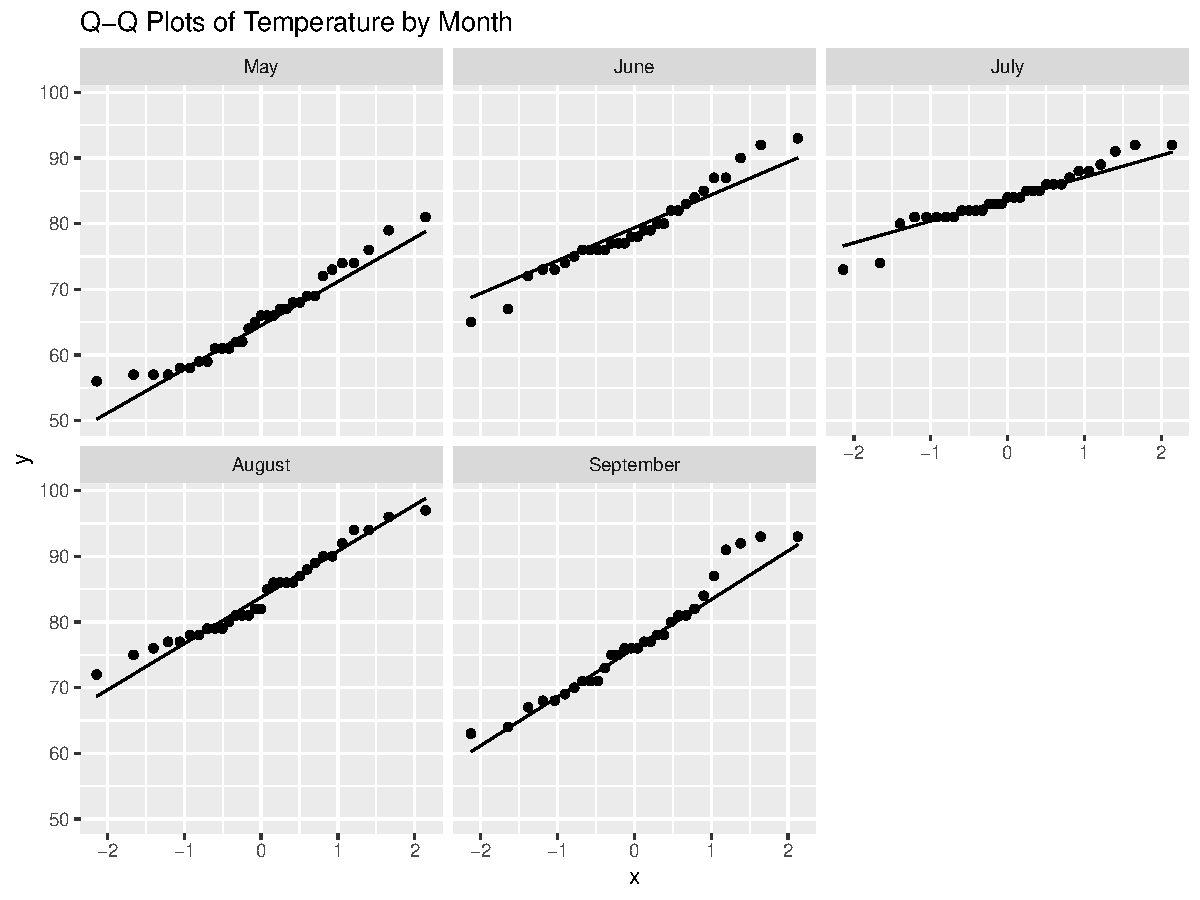
\includegraphics{question_7_files/figure-latex/unnamed-chunk-1-1.pdf}
\#\#\# a. Normality Test Results: The Shapiro-Wilk test was performed
for each month to test the normality of temperature distributions. A
p-value \textgreater{} 0.05 indicates normal distribution. Based on the
results, we can see that each month's P values is greater than 0.05.
Thus, it follows a normal distribution for each month.

\begin{enumerate}
\def\labelenumi{\alph{enumi}.}
\setcounter{enumi}{1}
\tightlist
\item
  Perform test of equality of variance on ``Temp'' variable by each
  category of Month variable and interpret the result carefully
\end{enumerate}

\begin{Shaded}
\begin{Highlighting}[]
\CommentTok{\# b. Test of equality of variance}
\CommentTok{\# Levene\textquotesingle{}s test}
\NormalTok{levene\_test }\OtherTok{\textless{}{-}} \FunctionTok{leveneTest}\NormalTok{(Temp }\SpecialCharTok{\textasciitilde{}}\NormalTok{ Month, }\AttributeTok{data =}\NormalTok{ airquality)}
\FunctionTok{print}\NormalTok{(}\StringTok{"}\SpecialCharTok{\textbackslash{}n}\StringTok{Levene\textquotesingle{}s Test for Equality of Variance:"}\NormalTok{)}
\end{Highlighting}
\end{Shaded}

\begin{verbatim}
## [1] "\nLevene's Test for Equality of Variance:"
\end{verbatim}

\begin{Shaded}
\begin{Highlighting}[]
\FunctionTok{print}\NormalTok{(levene\_test)}
\end{Highlighting}
\end{Shaded}

\begin{verbatim}
## Levene's Test for Homogeneity of Variance (center = median)
##        Df F value  Pr(>F)  
## group   4  2.5849 0.03941 *
##       148                  
## ---
## Signif. codes:  0 '***' 0.001 '**' 0.01 '*' 0.05 '.' 0.1 ' ' 1
\end{verbatim}

\subsubsection{b. Equality of Variance
Results:}\label{b.-equality-of-variance-results}

The Levene's test result (p-value = 0.03941 \textless{} 0.05) indicates
that the temperature variances are significantly different across
months. This means the spread of temperature values is not uniform
across all months - some months show more temperature variation than
others.

\begin{enumerate}
\def\labelenumi{\alph{enumi}.}
\setcounter{enumi}{2}
\tightlist
\item
  Compare Temp by Month using the best statistical test for this data
  and interpret the result carefully.
\end{enumerate}

\begin{Shaded}
\begin{Highlighting}[]
\CommentTok{\# c. ANOVA test}
\CommentTok{\# One{-}way ANOVA}
\NormalTok{anova\_result }\OtherTok{\textless{}{-}} \FunctionTok{aov}\NormalTok{(Temp }\SpecialCharTok{\textasciitilde{}}\NormalTok{ Month, }\AttributeTok{data =}\NormalTok{ airquality)}
\FunctionTok{print}\NormalTok{(}\StringTok{"}\SpecialCharTok{\textbackslash{}n}\StringTok{ANOVA Results:"}\NormalTok{)}
\end{Highlighting}
\end{Shaded}

\begin{verbatim}
## [1] "\nANOVA Results:"
\end{verbatim}

\begin{Shaded}
\begin{Highlighting}[]
\FunctionTok{print}\NormalTok{(}\FunctionTok{summary}\NormalTok{(anova\_result))}
\end{Highlighting}
\end{Shaded}

\begin{verbatim}
##              Df Sum Sq Mean Sq F value Pr(>F)    
## Month         4   7061  1765.3   39.85 <2e-16 ***
## Residuals   148   6557    44.3                   
## ---
## Signif. codes:  0 '***' 0.001 '**' 0.01 '*' 0.05 '.' 0.1 ' ' 1
\end{verbatim}

\subsubsection{c.~ANOVA Results:}\label{c.-anova-results}

The one-way ANOVA test was performed to compare mean temperatures across
different months. The F-statistic and p-value indicate whether there are
significant differences in temperature means across months. The ANOVA
results show a significant difference in mean temperatures across months
(p-value \textless{} 0.05). This suggests that at least one month's
temperature is significantly different from the others. However, ANOVA
does not specify which months differ, so a post-hoc test is necessary to
identify specific differences.

\begin{enumerate}
\def\labelenumi{\alph{enumi}.}
\setcounter{enumi}{3}
\tightlist
\item
  Perform the post-hoc test and interpret the results carefully
\end{enumerate}

\begin{Shaded}
\begin{Highlighting}[]
\CommentTok{\# d. Post{-}hoc analysis}
\CommentTok{\# Tukey\textquotesingle{}s HSD test}
\NormalTok{tukey\_result }\OtherTok{\textless{}{-}} \FunctionTok{TukeyHSD}\NormalTok{(anova\_result)}
\FunctionTok{print}\NormalTok{(}\StringTok{"}\SpecialCharTok{\textbackslash{}n}\StringTok{Tukey\textquotesingle{}s HSD Post{-}hoc Test Results:"}\NormalTok{)}
\end{Highlighting}
\end{Shaded}

\begin{verbatim}
## [1] "\nTukey's HSD Post-hoc Test Results:"
\end{verbatim}

\begin{Shaded}
\begin{Highlighting}[]
\FunctionTok{print}\NormalTok{(tukey\_result)}
\end{Highlighting}
\end{Shaded}

\begin{verbatim}
##   Tukey multiple comparisons of means
##     95% family-wise confidence level
## 
## Fit: aov(formula = Temp ~ Month, data = airquality)
## 
## $Month
##                         diff          lwr       upr     p adj
## June-May         13.55161290   8.84386422 18.259362 0.0000000
## July-May         18.35483871  13.68583759 23.023840 0.0000000
## August-May       18.41935484  13.75035372 23.088356 0.0000000
## September-May    11.35161290   6.64386422 16.059362 0.0000000
## July-June         4.80322581   0.09547713  9.510974 0.0430674
## August-June       4.86774194   0.15999325  9.575491 0.0388654
## September-June   -2.20000000  -6.94617992  2.546180 0.7038121
## August-July       0.06451613  -4.60448499  4.733517 0.9999995
## September-July   -7.00322581 -11.71097449 -2.295477 0.0006215
## September-August -7.06774194 -11.77549062 -2.359993 0.0005376
\end{verbatim}

\begin{Shaded}
\begin{Highlighting}[]
\CommentTok{\# Visual representation of results}
\FunctionTok{ggplot}\NormalTok{(airquality, }\FunctionTok{aes}\NormalTok{(}\AttributeTok{x =}\NormalTok{ Month, }\AttributeTok{y =}\NormalTok{ Temp, }\AttributeTok{fill =}\NormalTok{ Month)) }\SpecialCharTok{+}
  \FunctionTok{geom\_boxplot}\NormalTok{() }\SpecialCharTok{+}
  \FunctionTok{labs}\NormalTok{(}\AttributeTok{title =} \StringTok{"Temperature Distribution by Month"}\NormalTok{,}
       \AttributeTok{x =} \StringTok{"Month"}\NormalTok{,}
       \AttributeTok{y =} \StringTok{"Temperature (°F)"}\NormalTok{) }\SpecialCharTok{+}
  \FunctionTok{theme\_minimal}\NormalTok{()}
\end{Highlighting}
\end{Shaded}

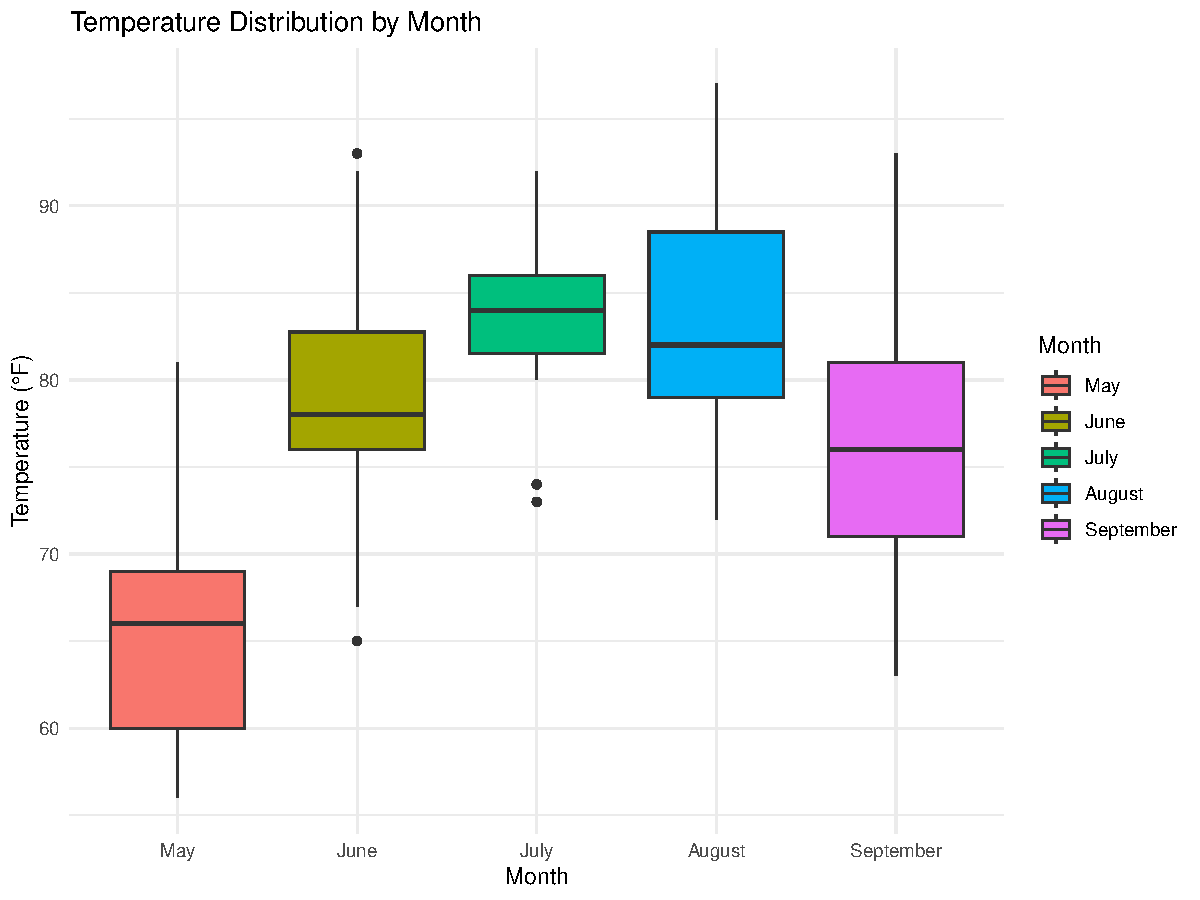
\includegraphics{question_7_files/figure-latex/unnamed-chunk-4-1.pdf}

\subsubsection{d.~Post-hoc Analysis
Results:}\label{d.-post-hoc-analysis-results}

Tukey's HSD test was performed to identify which specific months have
significantly different temperatures from each other. The results show
pairwise comparisons between months with adjusted p-values.

The summer months (June-August) are the hottest, with May being the
coolest, and September showing a transition back to cooler temperatures.

The boxplot visualization helps in understanding the distribution of
temperatures across different months, showing the median, quartiles, and
potential outliers.

\end{document}
